\documentclass[12pt]{article}
\usepackage{fullpage,enumitem,amsmath,amssymb,graphicx}
\usepackage{listings}
\usepackage{tikz}
\usepackage{hyperref}

\begin{document}

\begin{center}
{\Large CS 228 Winter 2018 Homework 1}

\begin{tabular}{rl}
SUNet ID: & 05794739 \\
Name: & Luis Perez \\
Collaborators: & \\
Late Days: & 2
\end{tabular}
\end{center}

By turning in this assignment, I agree by the Stanford honor code and declare
that all of this is my own work.

\section*{Problem 1}
It is good news that the disease is rare because, despite the high accuracy of the test, the rarity of the disease actually makes it quite unlikely that you have the disease (even after testing positive).

To see this, let $T$ be the even that the test is positive. Let $D$ be the event that you have the disease. Then we're interested in calculating $P(D \mid T)$, which by Bayes' rule, we can write as:
\begin{align*}
	P(D \mid T) &= \frac{P(T \mid D)P(D)}{P(T)} \\
	&= \frac{P(T \mid D)P(D)}{P(T \mid D)P(D) + P(T \mid \bar{D})P(\bar{D})} \\
	&= \frac{(0.99)(0.0001)}{(0.99)(0.0001) + (0.01)(0.9999)} \\
	&= \frac{1}{102} \approx 0.98\%
\end{align*}
Therefore, due to the rarity of the disease, even after testing positive, there's still slightly less than a $1\%$ chance that you actually have the disease (despite the ``high'' accuracy of the test).

\pagebreak

\section*{Problem 2}
We can use the Markov assumption directly to help us solve this problem. We first note that the problem consists of finding the maximum values of a joint distribution of $n$ random variables which all take values in the set $\mathcal{S}$. We can break the problem into the following:
\begin{align*}
\max_{x_1, \cdots, x_n \in \mathcal{S}^n} P(x_n, \cdots, x_1) &= \max_{x_1, \cdots, x_n \in \mathcal{S}^n} P(x_n \mid x_{n-1}, \cdots, x_1)P(x_{n_1}, \cdots, x_1) \tag{definition of joint distribution} \\
&=  \max_{x_1, \cdots, x_n \in \mathcal{S}^n} P(x_n \mid x_{n-1})P(x_{n_1}, \cdots, x_1) \tag{Markov assumption} \\
&=\max_{x_{n-1}, x_n \in \mathcal{S}^2} P(x_n \mid x_{n-1}) \max_{x_1, \cdots, x_{n-1} \in \mathcal{S}^{n-1}}P(x_{n-1}, \cdots, x_1) 
\end{align*}
From the above, we can immediately note that the problem consists of two simple steps:
\begin{enumerate}
\item Find the maximum values over the conditional distributions $P(X_i = u \mid X_{i-1} = v)$
\item Solve an instance of the same problem but only over $i - 1$ variables.
\end{enumerate}
We further note that in the base case where $i = 1$, we need only take the maximum over the values of the distribution $P(X_1 = x)$.

The above gives rise to the following algorithm, where $X1 \in [0,1]^m$ represents the distribution of $P(X_1 = v)$ and $Xi \in [0,1]^{m \times m}$ is the $m \times m$ matrix representing the conditional distributions $P(X_i = u \mid X_{i-1} = v)$.
\begin{lstlisting}[language=Python]
def Procedure(X1, X2, ..., Xn):
	res = max(X1)
	for i = 2 in 2...n:
		res *= max(Xn)
	return res
\end{lstlisting}
This very directly translates into a running time of $O(m + m^2(n-1)) = O(m^2n)$ since each iteration of the loop would take $O(m^2)$ to find the max over an $m \times m$ matrix.

\pagebreak
\section*{Problem 3}
It is simple enough to come up with a counter example. Consider the directed cyclic graph given by $G = (V,E)$ where $V = \{X_1, X_2, \cdots, X_n \}$ and $E = \{(X_1,X_2), (X_2,X_3),\cdots (X_{n-1}, X_n), (X_n,X_1) \}$. Now consider the conditional probability distributions which are fully determined by the value of the parent. Formally, these are defined as:
$$
f_v(x_v \mid x_{pa}(v)) = \begin{cases} 
    0 & x_v \neq x_{pa}(v) \\
    1 & x_v = x_{pa}(v)
 \end{cases}
$$
which are perfectly valid conditional distributions.

However, now consider summing over all values of the joint distribution.
\begin{align*}
\sum_{x_1, \cdots, x_n \in Val(X_1) \times \cdots \times Val(X_n) } f(x_1, \cdots, x_n) 
&= \sum_{x_1, \cdots, x_n \in Val(X_1) \times \cdots \times Val(X_n) } \prod_{v \in V} f_v(x_v \mid x_{pa}(v)) \\
&= \sum_{x_1 = x_2 = \cdots = x_n} 1 \tag{the conditional probability is $1$ only when the values are equal} \\
\end{align*}
For the above, we either have that the sum sums to $0$ (if $\bigcap_{v \in V} Val(X_v) = \emptyset$), the sum sums to $1$ (if $\left|\bigcap_{v \in V} Val(X_v) \right| = 1$), or the sum is larger than $1$ (all other cases). Note that in the latter case (which is simple enough to construct), we have an improper joint distribution. Therefore Bayesian networks must be defined as acyclic.

\pagebreak
\section*{Problem 4}
\begin{itemize}
  \item We wish to calculate $\Pr(\alpha \mid \beta, \gamma)$ and we have no conditional independence information. In this case, knowing:
  \begin{enumerate}[label=\arabic*.]
  	\item $\Pr(\beta, \gamma), \Pr(\alpha), \Pr(\beta \mid \alpha)$, and $\Pr(\gamma \mid \alpha)$ is not sufficient to calculate what we want since we cannot obtain the joint conditional distribution of $\beta, \gamma$ given $\alpha$ with only the given distributions. Without any conditional independence information, we have $\Pr(\beta, \gamma \mid \alpha) = \Pr(\beta \mid \gamma, \alpha)P(\gamma \mid \alpha)$.
  	\item $\Pr(\beta, \gamma), \Pr(\alpha)$ and $\Pr(\beta, \gamma|\alpha)$ are sufficient. We can directly calculate what we want using Bayes' Rule:
  	$$
  		\Pr(\alpha \mid \beta, \gamma) = \frac{\Pr(\beta, \gamma \mid \alpha)\Pr(\alpha)}{\Pr(\beta, \gamma)}
  	$$
  	\item $\Pr(\beta \mid \alpha), \Pr(\gamma \mid \alpha)$, and $\Pr(\alpha)$ is not sufficient to calculate what we want since we cannot obtain the joint conditional distribution of $\beta, \gamma$ given $\alpha$ with only the given distributions (see 1).
 	\end{enumerate}
  \item We now suppose we know that $\beta$ and $\gamma$ are conditionally independent given $\alpha$. We note that all sets can now be directly computed as follows, since we know that $\Pr(\beta, \gamma \mid \alpha) = \Pr(\beta \mid\alpha)\Pr(\gamma \mid \alpha)$.
  \begin{enumerate}[label=\arabic*.]
  	\item $\Pr(\beta, \gamma), \Pr(\alpha), \Pr(\beta \mid \alpha)$, and $\Pr(\gamma \mid \alpha)$ is sufficient.
  	\begin{align*}
			\Pr(\alpha \mid \beta, \gamma) &= \frac{\Pr(\beta, \gamma \mid \alpha)\Pr(\alpha)}{\Pr(\beta, \gamma)} \tag{Bayes' Rule} \\
			&= \frac{\Pr(\beta \mid \alpha)\Pr(\gamma \mid \alpha)\Pr(\alpha)}{\Pr(\beta, \gamma)} \tag{Conditional Independence}
  	\end{align*}
  	\item $\Pr(\beta \mid \alpha), \Pr(\gamma \mid \alpha)$, and $\Pr(\alpha)$ is sufficient to calculate what we want. It can be directly computed as follows (though note that this problem is likely computationally intractible):
  	\begin{align*}
			\Pr(\alpha \mid \beta, \gamma) &= \frac{\Pr(\beta, \gamma \mid \alpha)\Pr(\alpha)}{\Pr(\beta, \gamma)} \tag{Bayes' Rule} \\
			&= \frac{\Pr(\beta \mid \alpha)\Pr(\gamma \mid \alpha)\Pr(\alpha)}{\Pr(\beta, \gamma)} \tag{Conditional Independence} \\
			&= \frac{\Pr(\beta \mid \alpha)\Pr(\gamma \mid \alpha)\Pr(\alpha)}{\sum \Pr(\beta, \gamma \mid \alpha)P(\alpha)} \tag{Law of Total Probability} \\
			&= \frac{\Pr(\beta \mid \alpha)\Pr(\gamma \mid \alpha)\Pr(\alpha)}{\sum \Pr(\beta \mid \alpha)\Pr(\gamma \mid \alpha)P(\alpha)} \tag{Conditional Independence}
  	\end{align*}
 	\end{enumerate}
\end{itemize}

\pagebreak
\section*{Problem 5}
\begin{enumerate}
\item We directly compute the result:
\begin{align*}
\Pr(A = 0, B = 0) &= \Pr(A = 0 \mid B = 0) \Pr(B = 0) \\
&= \Pr(A = 0)\Pr(B = 0) \tag{$A$ and $B$ are independent since there are no active paths between them} \\
&= 0.8 * 0.3 \\
&= 0.24
\end{align*}
and
\begin{align*}
\Pr(E = 1 \mid A = 1) &=  \Pr(E = 1) \tag{$E \perp A$ since there are no active paths between $A$ and $E$} \\
&= \Pr(E = 1 \mid B = 1)\Pr(B=1) + \Pr(E = 1 \mid B = 0)\Pr(B=0) \tag{total probability}\\
&= 0.1(.7) + 0.9(0.3)\\
&= 0.34
\end{align*}
\item
\begin{enumerate}[label=(\alph*)]
\item False. There is an active path given by $A \to C \to F \to H \leftarrow E$ because $H$ is in the observed set.
\item True. There are only two paths between $G$ and $E$. The path $G \leftarrow F \leftarrow D \leftarrow B \to E$ is not active since $D$ is observed, and the path $G \leftarrow F \to H \leftarrow E$ is not active because $H$ is not observerd.
\item False. There is an active path given directly by $B \to E \to H$, therefore $\{A,B\}$ and $\{G,H\}$ are not d-sep given $F$.
\end{enumerate}
\end{enumerate}

\pagebreak
\section*{Problem 6}

\begin{enumerate}
\item The expected Creativity score of a student is given by:
\begin{align*}
E[C] &= \int_{0}^1 c f_C(c) dc \\
&= \int_0^1 c dc \tag{$f_C(c) = 1$} \\
&= \frac{c^2}{2}\big\vert_0^1 \\
&= \frac{1}{2} 
\end{align*}
\item The expected Creativity score of an admitted student can be calculated in two equivalent methods. We present both. In the first method, we consider the joint distribution $f(c,i)$ over both $C$ and $I$ which is a uniform distribution over the unit square. Therefore, to determine the expected value of $C$ we simply need to integrate the distribution times $c$ over the subset defined by $I + C \geq 1.5$ and re-normalize. This directly gives us:
\begin{align*}
E[C \mid C + I \geq 1.5] &= \frac{\int_{0.5}^1\int_{1.5 - c}^1 c dIdC}{\int_{0.5}^1\int_{1.5 -c}^1dI dC} \\
&=\frac{\int_{0.5}^1c(c-0.5)dC}{\int_{0.5}^1 (c- 0.5) dC} \\
&= \frac{\frac{5}{48}}{\frac{1}{8}} \\
&= \frac{5}{6}
\end{align*}
We can arrive at the same conclusion using a slighty different method. We note that:
\begin{align*}
f_{C \mid C + I > 0.5}(c) &= \frac{f_{C+I \geq 1.5 \mid C}(c)f_{C}(c)}{f_{C + I \geq 1.5}(c)} \\
&= \frac{c-0.5}{\int_{0.5}^1 (c- 0.5) dC} \\
&= 8(c - 0.5) \tag{zero where $c \notin [0.5, 1]$}
\end{align*}
We can then use the above result to calculate the expected valued directly:
\begin{align*}
E[C \mid C + I \geq 1.5] &= \int_{0}^1 c f_{C \mid C + I \geq 1.5}(c) dC \\
&= 8\int_{0.5}^1 c(c-0.5) dC \\
&= 8*\frac{5}{48} \\
&= \frac{5}{6}
\end{align*}

\item The expected Creativity score of a student with $I = 0.95$ is:
$$
E[C \mid I = 0.95] = E[C] = 0.5
$$
since $C \perp I$ so knowing $I = 0.95$ gives no information about $C$.
\item The expected Creativity score of an admitted student with $I = 0.95$ is given by (following method $1$ as discussed above):
\begin{align*}
E[C \mid C + I \geq 1.5, I = 0.95] &= E[C \mid C \geq 0.55] \\
&= \frac{\int_{0.55}^1 c dC}{\int_{0.55}^1 dC} \\
&= 0.775
\end{align*}
We note that the expected creativity of an admitted student with high intelligence is actually lower than the expected creativity of an admitted student. While at first counter-intuitive, this makes sense if we consider the fact that admitted students must have $C + I \geq 1.5$. This means that high intelligence, for the population of admitted students, is actually correlated with lower creativity (since intelligence alone might have been sufficient to admit them, creativity does not need to be as high). To make this more concrete, consider any students with Creativity $0.5$ (the lowest possible, given they are admitted). These students must necessarily have $I = 1$. Therefore, the only students with the lowest creativity score are those that have the highest possible intelligence.
\end{enumerate}

\pagebreak

\section*{Problem 7}
\begin{enumerate}
\item We construct a Bayesian network without Alarm as shown in Figure \ref{fig:reduced_bayesian_network} where we use the first letter of the event to name each node. 
The network we constructed has two requirements: (1) $I(G') \subseteq I(G)$ (we must not introduce any new independences) and (2) it must be minimal. In order to achive (1), note that we require $X \perp Y \mid Z \in I(G') \implies X \perp Y \mid Z \in I(G)$ which is equivalent to $d_{sep}^{G'}(X;Y\mid Z) = true \implies d_{sep}^{G}(X;Y\mid Z) = true$ which is equivalent to $d_{sep}^G(X;Y \mid Z) = false \implies d_{sep}^{G'}(X;Y \mid Z) = false$. If we satisfy the above, we know that $(1)$ is satisfied. Therefore, we are interested in first enumerating which triplets $X,Y,Z$ are not $d$-seperated in $G$ (where $X,Y,Z \neq A$). We have:

\begin{itemize}
\item $B,J$ always have an active path between them (again, recall we don't consider triplets with $A$) and are therefore never $d$-seperated.
\item Similarly, $B,M$ are never $d$-seperated.
\item $B,T$ are not $d$-seperated only when we observe $J$ (due to the v-structure).
\item $B,N$ are not $d$-seperated only when we observe $M$.
\end{itemize}
Symetrically, this holds when replacing $B$ with $E$. All other triplets are always $d$-seperated.

From the above, we see that by removing $A$ we must:
\begin{itemize}
\item We must have at least one direct edge connecting $B$ to $J$ and $M$ as similarly for $E$. Otherwise, if all paths connecting these have an intermediary node, then there exists a set of observable variables that would introduce $d$-seperate them.
\item Addressed above.
\item Due to the v-structure around $J$, $B,T$ and $B,M$ are always $d$-seperated unless we observe $J$.
\item Similar argument to above.
\end{itemize}

The next step is demonstrating that this map is minimal. We can do this by considering the removal of each edge and showing that this introduces new conditional independences. If we remove $B,J$ we introduce $B \perp J \mid E$, symetrically for removing $E,M$. If we remove $B,M$, we introduce $B \perp M \mid E$ (symetrically for removing $E,J$). The other edges are the same as in the original graph, so we cannot remove them. 

With the above, we satisfy $(1)$ and $(2)$, thereby showing this is a minimal I-map.


\begin{figure}[h!]
\centering
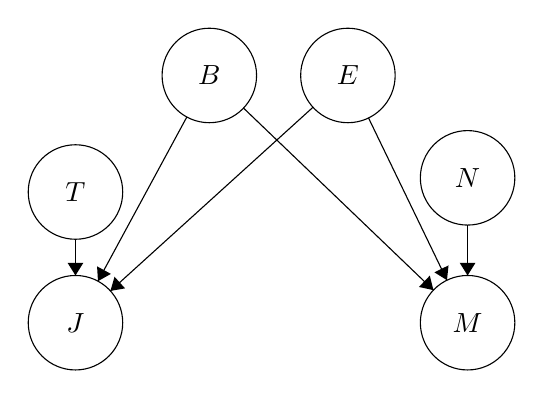
\begin{tikzpicture}[scale=0.2]
\tikzstyle{every node}+=[inner sep=0pt]
\draw [black] (32,-7.9) circle (3);
\draw (32,-7.9) node {$B$};
\draw [black] (23.5,-15.3) circle (3);
\draw (23.5,-15.3) node {$T$};
\draw [black] (40.8,-7.9) circle (3);
\draw (40.8,-7.9) node {$E$};
\draw [black] (48.4,-14.4) circle (3);
\draw (48.4,-14.4) node {$N$};
\draw [black] (48.4,-23.6) circle (3);
\draw (48.4,-23.6) node {$M$};
\draw [black] (23.5,-23.6) circle (3);
\draw (23.5,-23.6) node {$J$};
\draw [black] (34.17,-9.97) -- (46.23,-21.53);
\fill [black] (46.23,-21.53) -- (46,-20.61) -- (45.31,-21.33);
\draw [black] (38.58,-9.92) -- (25.72,-21.58);
\fill [black] (25.72,-21.58) -- (26.65,-21.42) -- (25.98,-20.68);
\draw [black] (30.57,-10.54) -- (24.93,-20.96);
\fill [black] (24.93,-20.96) -- (25.75,-20.5) -- (24.87,-20.02);
\draw [black] (42.11,-10.6) -- (47.09,-20.9);
\fill [black] (47.09,-20.9) -- (47.19,-19.96) -- (46.29,-20.4);
\draw [black] (23.5,-18.3) -- (23.5,-20.6);
\fill [black] (23.5,-20.6) -- (24,-19.8) -- (23,-19.8);
\draw [black] (48.4,-17.4) -- (48.4,-20.6);
\fill [black] (48.4,-20.6) -- (48.9,-19.8) -- (47.9,-19.8);
\end{tikzpicture}
\centering
\caption{Minimal I-Map of Bayesian Network}
\label{fig:reduced_bayesian_network}
\end{figure}

\item We can simplify this problem greatly by first considering the Markov blanket of $X_i$, defined as $M(X_i)$ as the set of parents, children, and parents of children of $X_i$. Let $G = (V, E)$ be the directed graph representing the Bayesian network. Then recall that $P(X_k \mid X_i, M(X_i)) = P(X_k \mid M(X_i))$ for all $X_k \in V \setminus (M(X_i) \cup X_i)$. This means that the removal of $X_i$ should have no affect on any nodes outside $M(X_i)$.

We now consider the following algorithm:
\begin{itemize}
\item For all nodes in the Markov blanket, find all pairs such that $X_k \perp X_j$ such that without consider $X_i$, they always have an active path between them.
\item For these tuples, form an edge $(X_k, X_j)$ in the natural ordering (the parent of $X_i$ becomes the parent of the child of $X_i$).
\end{itemize}
\end{enumerate}

\pagebreak
\section*{Problem 8}

\begin{enumerate}
\item We wish to compute $P(x_i \mid x_1, \cdots, x_{i-1}, x_{i+1}, \cdots, x_n)$ where all variables except $X_i$ have been observed. We work from first principles (though part of this will repeat what we learned about Markov blankets). We first define $\pi(i)$ as the set of parent nodes of $X_i$, $C(i)$ as the set of children nodes of $X_i$, $\pi(C(i))$ as the set of parents of children of $X_i$ (excluding $X_i$), and $O(i)$ as everything outside the Markov blanket of $X_I$, formally defined as $O(i) = V \setminus[\pi(i) \cup C(i) \cup \pi(C(i)) \cup \{X_i\}]$. We are somewhat lose in our notation (for succincness). With the above definitions, we have:

\begin{align*}
P(x_i \mid x_1, \cdots, x_{i-1}, x_{i+1}, \cdots, x_n) &= P(X_i \mid O(i), \pi(i), C(i), \pi(C(i))) \tag{definition plus some lose notation} \\
&= \frac{P(X_i, O(i), \pi(i), C(i), \pi(C(i))}{\sum_{x_i} P(X_i, O(i), \pi(i), C(i), \pi(C(i))} \tag{Bayes Rule} \\
&= \frac{P(X_i \mid \pi(i))P(C(i) \mid X_i, \pi(C(i)))P(\pi(i), \pi(C(i)), O(i))}{\sum_{x_i} P(X_i \mid \pi(i))P(C(i) \mid X_i, \pi(C(i)))P(\pi(i), \pi(C(i)), O(i))} \tag{Partial application of Chain rule on structure of network} \\
&= \frac{P(X_i \mid \pi(i))P(C(i) \mid X_i, \pi(C(i)))}{\sum_{x_i}P(X_i \mid \pi(i))P(C(i) \mid X_i, \pi(C(i)))}
\end{align*}
Note that the above is somewhat loose with notation, but points us to the direction of an efficient algorithm. More formally, the algorithm will first compute the below formula, for all $x_i \in Val(X_i)$:
\begin{align*}
P(x_1, \cdots, x_{i-1}, x_{i+1} \cdots x_n) &= \frac{1}{Z} P(X_i = x_i \mid \pi(i)) \prod_{c \in C(i)} P(X_c = x_c \mid \pi(c))
\end{align*}
We note that $P(x_i \mid \pi(i))$ and $p(x_c \mid \pi(c))$ are given by the network. Also note that $X_i \in \pi(c)$. Let us suppose that $|Val(X_k)| = d$ for all $k$. The algorithm begins for a given value $x_i$ by:
\begin{itemize}
\item Looking up $P(X_i = x_i \mid \pi(i))$ since all $\pi(i)$ are known.
\item Using $x_i$ and the other known values, looking up $P(X_c = x_c \mid \pi(c))$ for all $|C(i)|$ children of $X_i$.
\item Multiplying all the above together to obtain $P(X_i = x_i \mid X_{-i})$.
\end{itemize}
We must repeat the above process $d$ times (for each value of $x_i$) in order to obtain the full distribution, giving a total running time of $O(d|C(i)|)$. We note that $|C(i)| = O(n)$, so we have $O(dn)$ running time. Once we have the full distribution, we can simply normalize the vector which consists of summing $d$ values, so this takes $O(d)$ time. Therefore the algorithm has a running time of $O(d|C(i)|) = O(dn)$ to compute the conditional distribution of $x_i$ given all other seen variables. 

\item We show an efficient algorithm for sampling from a Bayesian network $G = (V,E)$. Following the hint, we first note that, in general, sampling from a join distribution can easily be accomplished by sampling from the conditional distributions. The process is as follows, for $(x,y) \sim P(X,Y)$:
\begin{itemize}
\item We note that $P(X,Y) = P(X)P(Y \mid X)$ by definition.
\item Sample $x \sim P(X)$.
\item Consider the conditional distribution $P(Y \mid X = x)$. Sample from this distribution $y \sim P(Y \mid X= x)$ where $x$ is the value sampled from $P(X)$.
\item By the definition presented, $(x,y) \sim P(X,Y)$.
\end{itemize}

We can make use of the above in sampling from a Bayesian network. Suppose $V = \{X_1, \cdots, X_n\}$ where the variables are ordered topologically. If they are not given in this order, note that we can determine the ordering in $O(|V| + |E|)$ times (linear in size of the network) by using DFS (for more details, see \href{https://en.wikipedia.org/wiki/Topological_sorting}{here}) This means that for every directed edge $X_u \to X_v$, $u < v$. Then we present the algorithm:
\begin{lstlisting}[language=Python]
def SampleNetwork(X1, X2, ..., Xn):
	res = 1
	samples = []
	for i = 1 to n:
	  x <- P(Xi | pa(Xi))
	  res *= x
	  samples[i] = x
return res
\end{lstlisting}
We first note that due to the fact that we're processing nodes in topological order, we always have that $pa(i) \subseteq \{X_k\}_{k < i}$. Therefore at iteration $i$, we have already sampled from $P(X_k \mid pa(k))$ for all $k < i$, and can directly sample from the conditional distribution given by the Bayesian network. Finally, we note that at the end of the loop, we will have:
$$
res = \prod_{i=1}^{n}P(X_i \mid pa(i)) = P(X_1, \cdots, X_n)
$$
\end{enumerate}

\pagebreak
\section*{Problem 9}

\begin{enumerate}
\item The random vector $X_{1:784}$ can take $2^{784} \approx 1.02e236$ possible values.
\item You would need $2^{784} - 1$ paramaters to specify an arbitrary probability distribution over the images.
\item We note that the joint distribution factorizes as:
$$
P(Z_1, Z_2, X_1, \cdots, X_{784}) = P(Z_1)P(Z_2)\prod_{i=1}^{784}P(X_i \mid Z_1, Z_2)
$$
We further note that $|Val(Z_i)| = 25$, so you need $2(25-1) = 48$ parameters to specify $P(Z_1)$ and $P(Z_2)$. For each of $P(X_i \mid Z_1, Z_2)$, a total of $25*25 - 1 = 624$ parameters are needed (this is becase knowing $P(X=1 \mid Z_1, Z_2$ also lets us know $P(X = 0 \mid Z_1, Z_2)$). This means the conditional distributions need a total of $624 * 784 = 489,216$ parameters to be specified, bringing the grand total for the network to $489,264 \approx 0.5M$.
\item We show the five samples in Figure 
\begin{figure}[h!]
\centering
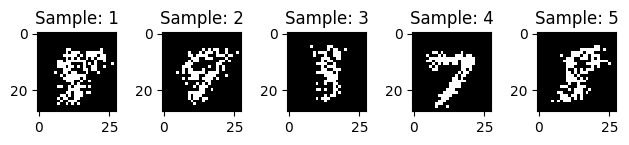
\includegraphics[scale=0.8]{programming/a4.png}
\caption{Sampled Digits from Model}
\label{fig:sampled_digits}
\end{figure}

\item We show the plot as we vary $Z_1$ and $Z_2$ in Figure \ref{fig:latent_variables}.
\begin{figure}[h!]
\centering
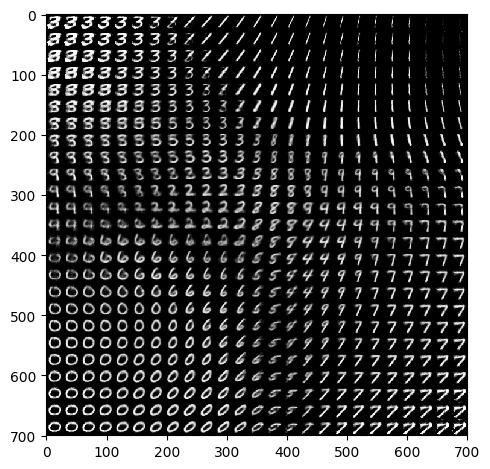
\includegraphics[scale=0.8]{programming/a5.png}
\caption{Exploring Space of Latent Variables}
\label{fig:latent_variables}
\end{figure}

The intuitive role for $Z_1$ (x-axis) appears to indicate how circular the value is (from 0 to 7 and from 3 to black). $Z_2$ on the other hand is more difficult to tell intuitively, though it appears to determine the horizontal width/lines.

\item We include the histograms of the marginal log likelihood $\log p(x_{1:784})$ for the real (Figure \ref{fig:hist_real}) and the corrupted data (Figure \ref{fig:hist_corrupted}).
\begin{figure}[h!]
\centering
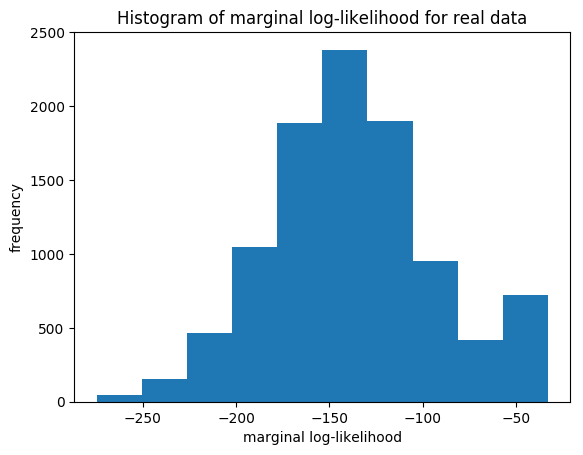
\includegraphics[scale=0.8]{programming/a6_hist_real.png}
\caption{Histogram of Marginal Log Likelihood for Real Images}
\label{fig:hist_real}
\end{figure}
\begin{figure}[h!]
\centering
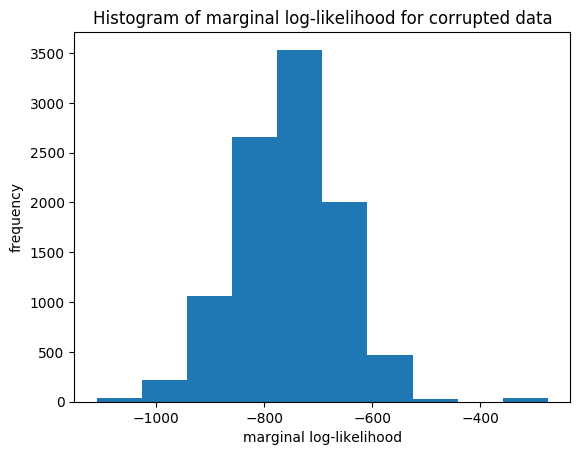
\includegraphics[scale=0.8]{programming/a6_hist_corrupt.png}
\caption{Histogram of Marginal Log Likelihood for Corrupted Images}
\label{fig:hist_corrupted}
\end{figure}

\item We first note that we can use Bayes rule to simplify the computation:
$$
p((Z_1, Z_2) = (z_1, z_2)|X_{1:784} = I^k) \propto p(X_{1:784} = I^k \mid (Z_1, Z_2) = (z_1, z_2))p((Z_1, Z_2) = (z_1, z_2))
$$
We can easily compute the above for all values of $z_1, z_2$, and we plot them along with their labels colored. We can see this in Figure \ref{fig:plot}. By Bayes Rule’, the posterior probability is directly proportional to the likelihood which leads
to a similar clustering of points for the conditional expectations in part 5 and 7. The mapping is not perfect, but we can see that $0$ and $7$ and other similar numbers tend to generally be in the same orientation in the graph.

\begin{figure}[h!]
\centering
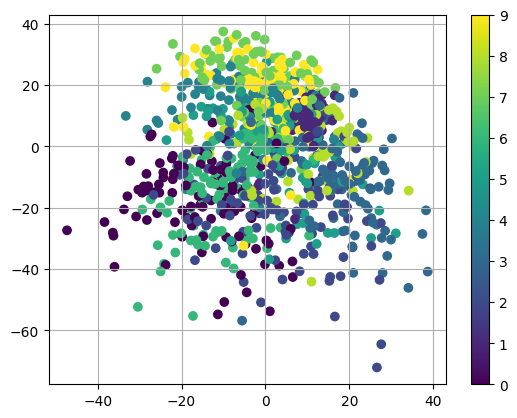
\includegraphics[scale=0.8]{programming/a7.png}
\caption{$E[Z_1 \mid X_{1:784}]$ by $E[Z_2 \mid \mid X_{1:784}]$}
\label{fig:plot}
\end{figure}

\end{enumerate}
\end{document}
